% \newcommand\tab[1][0,4cm]{\hspace*{#1}}
\newcommand\longtab[1][1cm]{\hspace*{#1}}
% \setlength{\headheight}{15pt}

\chapter{Generalités sur les applications mobiles}
\section{Introduction au sujet}
\newpage
\section{Solutions déja existantes}
\paragraph*{}
Il existe peu d'applications mobiles dans le domaine de la restauration nous allons explorer certaines des plus populaires solutions existantes aujourd’hui.


\subsection{TripAdvisor}
\begin{wrapfigure}[8]{r}{2cm}
    \vspace{-15pt}
    
\includegraphics[width=2cm]{images/Chapitre1/tripadvisor.png}
    \vspace{-20pt}
    \caption{{\footnotesize Logo de TripAdvisor}}
\end{wrapfigure}

TripAdvisor est une plate-forme disponible en web et en application mobile, cette plate-forme offre des avis et des suggestions d'hôtels, lieux de loisirs, villes et régions à l'échelle internationale, compare les prix et affiche les meilleures offres du moment.

TripAdvisor couvre aussi les services de restauration et fournit des informations sur les différents restaurants qui existent dans le monde entier. \bigskip

Le service qu'offre cette plate-forme pour le secteur de la restauration a des avantages : \bigskip

	\tab- L'utilisation de ce service est gratuite.\medskip

	\tab- Donne un aperçu sur les restaurants et offre des informations sur la fourchette des prix..\medskip

	\tab- Des évaluations et des avis sont fournis par les utilisateurs eux-mêmes.\bigskip

TripAdvisor a ses avantages mais aussi ses inconvénients:\bigskip

	\tab- On ne peut pas parcourir les restaurants en utilisant une carte géographique.\medskip

	\tab- L'utilisation d'une application tierce est indispensable pour avoir l'itinéraire vers les restaurants.\medskip

	\tab- Les informations offertes par cette plate-forme sont limitées au avis fourni par les utilisateurs.
 

	\begin{figure}[!ht]

		\centering
		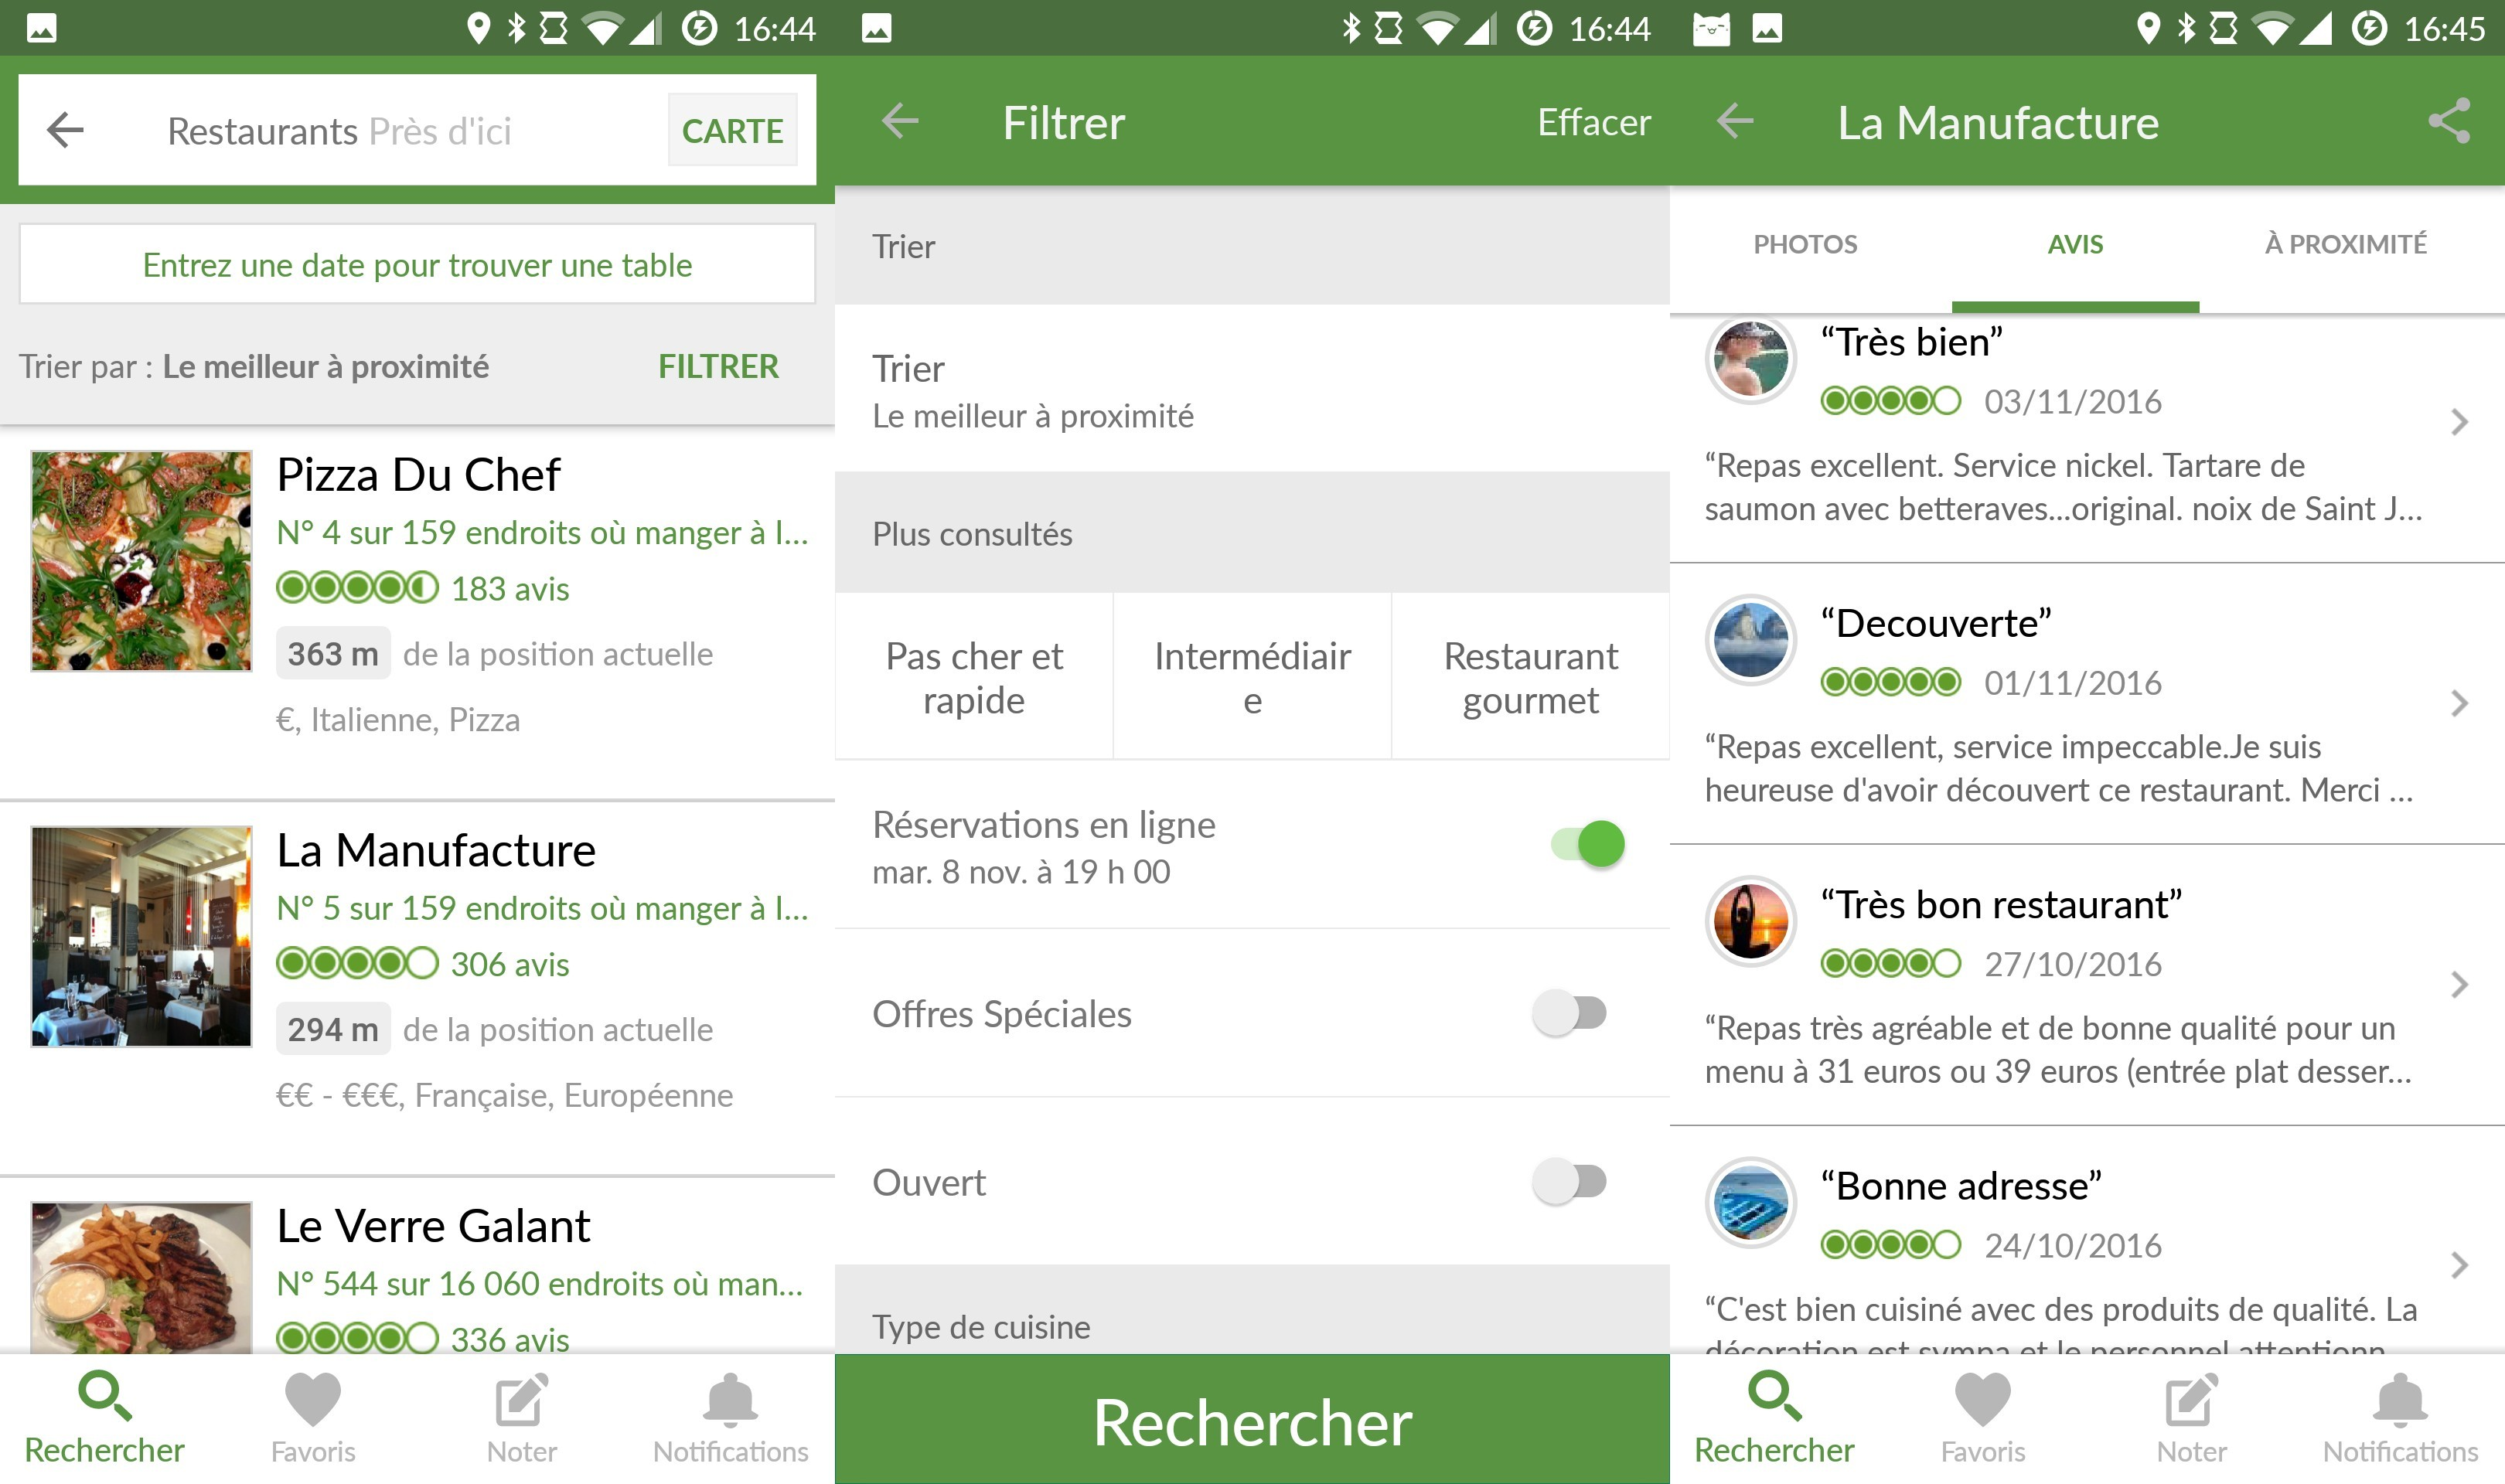
\includegraphics[width=4in]{images/Chapitre1/trip_advisor.jpeg}
		\label{fig:label}
		\caption{Interface de TripAdvisor lors de la recherche des restaurants et les avis}
	 \end{figure}
\newpage
\subsection{Google Maps}
\begin{wrapfigure}[8]{r}{2cm}
	\vspace{-15pt}
	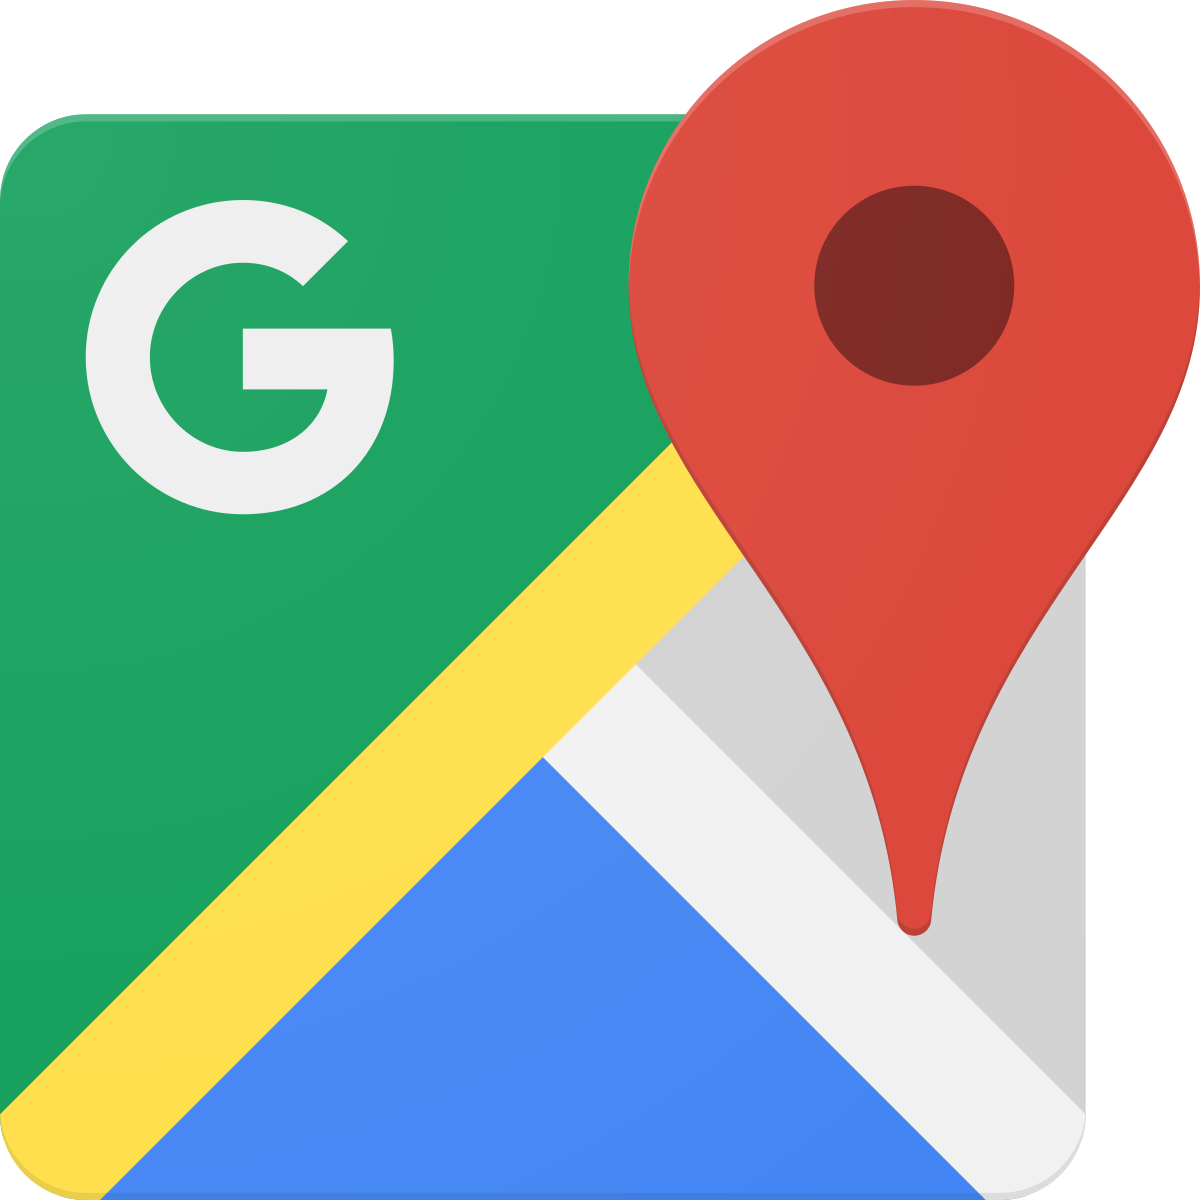
\includegraphics[width=2cm]{images/Chapitre1/googlemaps.png}
	\vspace{-20pt}
	\caption{{\footnotesize Logo de Google Maps}}
 \end{wrapfigure}
Google maps est un service de cartographie développé par l'entreprise Google et lancé en 2005. Ce service offre différents types de vues et permet aussi d'afficher les différents points d'intérêts dans le monde comme les hôtels, les lieux d'attractions, etc. Ce qui nous intéresse dans notre domaine de recherche est la géolocalisation des restaurants, une fonctionnalité qu'offre ce service.

En accédant au site web ou l'application mobile, l'utilisateur aura accès à un large choix de restaurants proposés grâce à un système de suggestions, aussi développé par Google. L'utilisateur pourra donc accéder aux informations des restaurants ainsi que des photos et des avis généralement postés par la communauté des utilisateurs de Google Maps.
\subparagraph*{}
Google Maps présente de nombreux avantages, nous en citerons :\bigskip
 
	\tab- L'utilisation de ce service est gratuite.\medskip

	\tab- La plupart des restaurants sont affichés dans la carte.\medskip

	\tab- Les images des restaurants sont parfois affichées.\medskip
	
	\tab- Les utilisateurs peuvent donner des avis et des notes.\medskip

	\tab- Des itineraires precis sont proposés.\bigskip

	
Néanmoins ce service présente aussi des inconvénients:\bigskip

	\tab- Les menus detaillés ne sont pas affichés dans l'interface.\medskip

	\tab- On ne peut pas filtrer les types de restaurants.\medskip


	\begin{figure}[!ht]

		\centering
		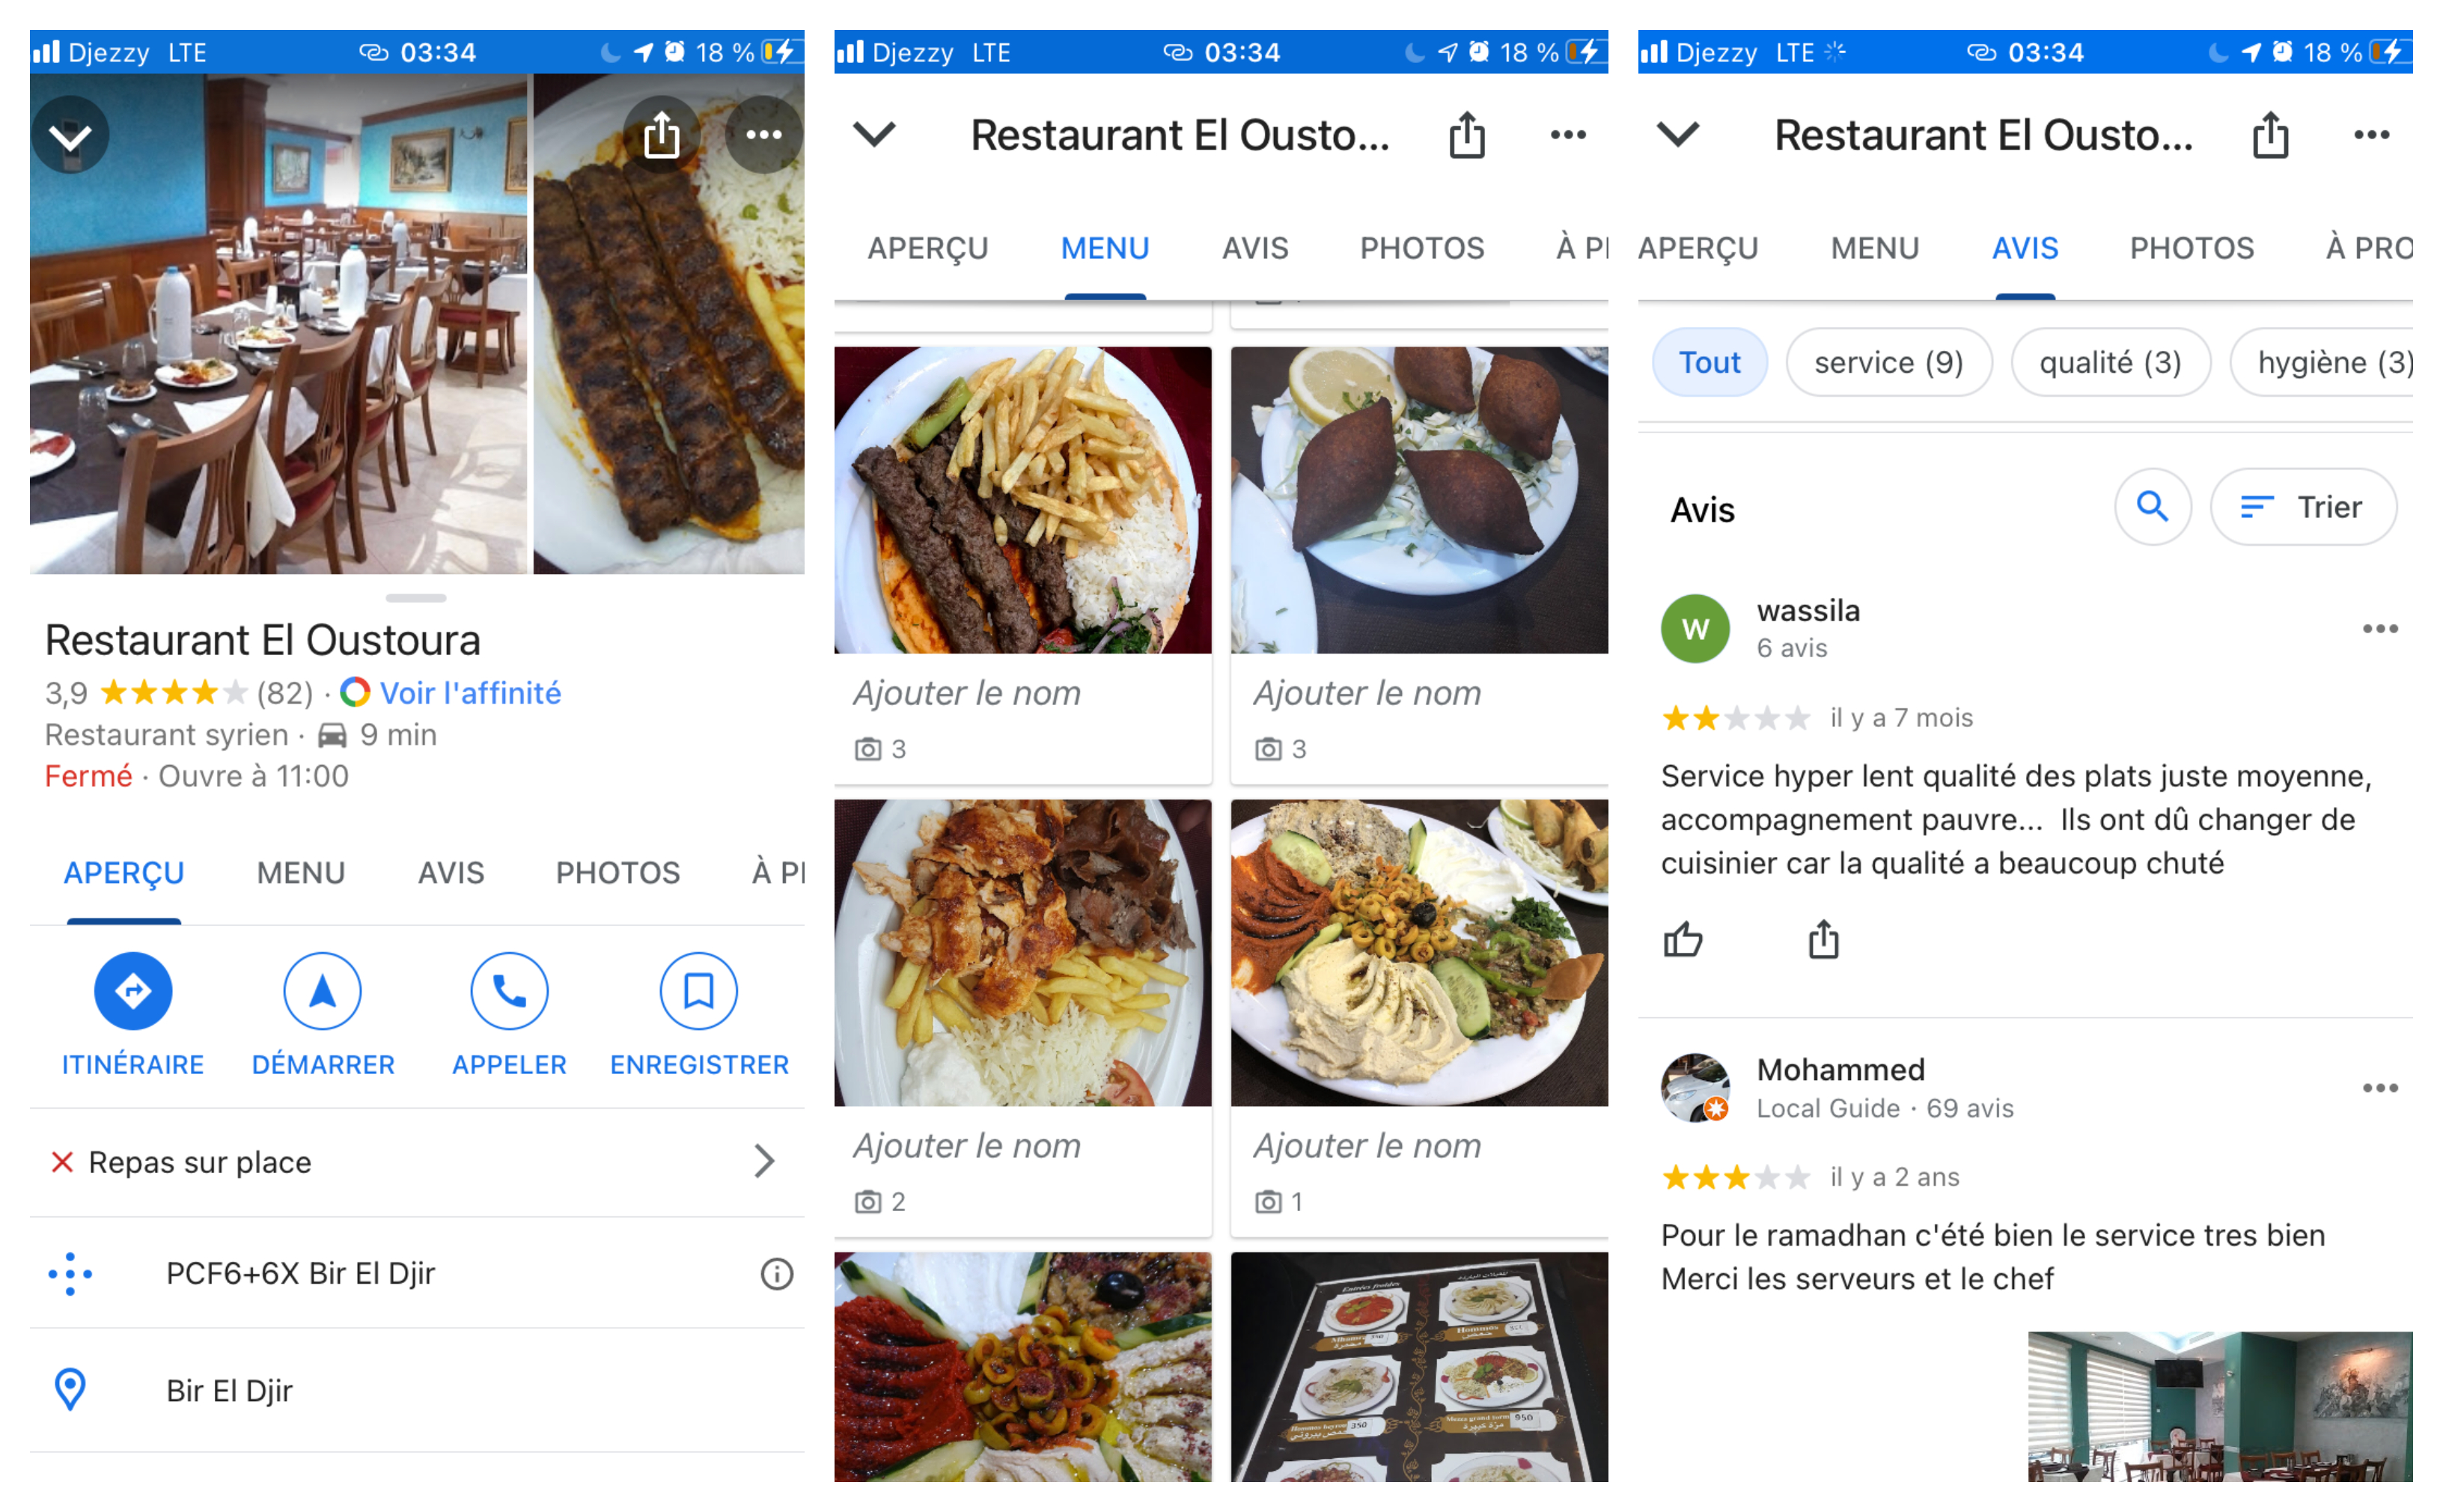
\includegraphics[width=4.5in]{images/Chapitre1/page_resto.jpg}
		\label{fig:label}
		\caption{Exemple de différents ecrans lors d'une recherche d'un restaurant }
	 \end{figure}
	 
\newpage

\subsection{LaFourchette}
TheFork de son ancien nom "LaFourchette" est une plate-forme française de réservation de restaurants en ligne, accessible par un site web et par une application mobile disponible sur Android et iOS. Elle est présente dans plus de vingt pays en Europe et en Amérique latine.~\cite{TheFork2020}
\subparagraph*{}
\begin{wrapfigure}[8]{r}{3cm}
    \vspace{-15pt}
    
\includegraphics[width=3cm]{images/Chapitre1/lafourchette.jpg}
    \vspace{-20pt}
    \caption{{\footnotesize Logo de LaFourchette}}
\end{wrapfigure}

\subparagraph*{}
TheFork a ces avantages et ces inconvénients, parmi ces avantages on a :\bigskip

	\tab- La base de données regroupe plus de 80000 restaurants a travers le monde.~\cite{RestaurantsSiteReservation} \medskip

	\tab- L'application est multiplate-forme et disponible en version web et mobile. \medskip

	\tab- L'interface utilisateur est simple qui permet d'utiliser le service de manière efficace. \medskip

	\tab- La présence de la fonction d'exploration des restaurants via une carte.\bigskip

Quant aux Inconvénients nous citeront :\bigskip

	\tab- Le service n'est pas totalement gratuit.\medskip

	\tab- Cette application est dédiée qu'aux réservations de restaurans et ne donne pas des informations détaillées sur les menus.\medskip

	\tab- L'application ne prends pas encore en charge les restaurans algeriens. \medskip

   



\newpage
\subsection{Wahrfood}

\subparagraph*{}
\begin{wrapfigure}[8]{r}{3cm}
	\vspace{-15pt}
	\begin{flushright}

\includegraphics[width=3cm]{images/Chapitre1/wahrfood.jpg}
	\end{flushright}
    \vspace{-20pt}
    \caption{{\footnotesize Logo de Wahrfood}}
\end{wrapfigure}
\begin{list}{•}{\textbf{Avantages}}
	\item - L'utilisation est gratuite 
	\item - Disponible sous IOS et Android 
	\item - On peut livrer des commandes directement 
	\item - explorer les restaurants a proximité
	
\end{list}

\subparagraph*{}
\begin{list}{•}{\textbf{Inconvénients}}
	\item - Il faut avoir un compte pour voir le contenu 
	\item - pas de version web 
	\item - Une expérience utilisateur moyenne.
	\item - On ne peut pas avoir les restaurant dans une carte
   
\end{list}

\newpage
\subsection{Les reseaux sociaux }

\subparagraph*{}
\begin{wrapfigure}[8]{r}{3cm}
	\vspace{-15pt}
	\begin{flushright}

\includegraphics[width=3cm]{images/Chapitre1/wahrfood.jpg}
	\end{flushright}
    \vspace{-20pt}
    \caption{{\footnotesize Logo de Wahrfood}}
\end{wrapfigure}
\begin{list}{•}{\textbf{Avantages}}
	\item - L'utilisation est gratuite 
	\item - Disponible sous IOS et Android 
	\item - On peut livrer des commandes directement 
	\item - explorer les restaurants a proximité
	
\end{list}

\subparagraph*{}
\begin{list}{•}{\textbf{Inconvénients}}
	\item - Il faut avoir un compte pour voir le contenu 
	\item - pas de version web 
	\item - Une expérience utilisateur moyenne.
	\item - On ne peut pas avoir les restaurant dans une carte
   
\end{list}
\newpage
\section{Solutions Proposées}
bezef hedra
\newline
La solution consiste en une application mobile 
fonctionnant sur Android et IOS ou les utilisateurs
sont capable de : 
\begin{list}{•}{}
\item 
\end{list}
